\section{Grafisk bruger interface}\label{GUI_design}
\textit{Dette afsnit omhandler design, implementering og test af Graphical User Interface (GUI) til visualisering af de udførte aktiviteter. Først designes GUI til det specifikke formål ud fra dets kravspecifikationer, hvorefter denne kan implementeres. Afslutningsvist bliver GUI testet i forhold til opstillede krav, som beskrevet i \secref{krav_GUI}.}

\subsection{Design}
GUI benyttes til at motivere børn til en mere aktiv hverdag. Dette gøres ud fra \secref{motivation_boern}, hvor det beskrives at børn motiveres gennem succesoplevelser. GUI designes med henblik på at give børnene et overblik over hvor lang tid de har udført en given aktivitet, og hvor mange point de har optjent som følge af dette. Pointene vægtes ud fra aktivitetstypen og varigheden heraf. 

Data fra algoritmerne vedrørende aktiviteterne gang og løb, samt data fra gyroskopet sendes til MATLAB i form af et array med tre variable. Den første variabel består af en identifikation (ID), hvormed det kan identificeres hvorvidt data kommer fra accelerometeret eller gyroskopet, som det ses på \figref{fig:GUI}. Id for accelerometeret er to, mens ID for gyroskopet er tre.\\
Registreres ID for accelerometeret er der på anden plads i arrayet en peakværdi, som informerer om hvilken aktivitet varigheden bør tillægges. På tredje plads er der et resultat af varighed siden sidst detekterede peak. Er peakværdien mellem 100 og 1100 skal varigheden lægges i tidsvariablen for gang, og er den over 1100 skal den lægges over i tidsvariablen for løb.\\
Registreres ID for gyroskopet, tillægges anden værdi i arrayet for fra mikrokontrolleren i et array for gyroskopet, som er i MATLAB, hvorefter signalbehandlingen, som er beskrevet i \secref{sec:algocykel}. Giver denne værdi over 70 \% overføres fire sekunder til tidsvariablen for cykling, eftersom signalbehandlingen er foretaget over samplings af denne varighed. På den tredje plads i arrayet er repræsenteret tallet fire, som ikke bruges i nogen beregninger, denne er til for at mikrokontrollerens array for alle tre aktiviteter er lige lange. 

Hver aktivitet belønnes forskelligt, da det er væsentligt at få børnene til at løbe og cykle mere, end at gå. Dermed multipliceres tiden for løb med tre, for cykling med to og for gang med en. Pointene visualiseres ud for den enkelte aktivitet, så barnet kan se hvor mange point de har opnået ved udførslen for den enkelte aktivitet igennem en hel dag. For at aktivere børnene hver dag, samles dagens point for alle aktiviteter udført i løbet af dagen. Pointene vises grafisk som en søjle hvormed barnet kan få et overblik over antallet af point fra de forskellige dage, samt hvor stor en del der er opnået ved henholdsvis gang, løb og cykling.  

\begin{figure}[H]
	\centering
	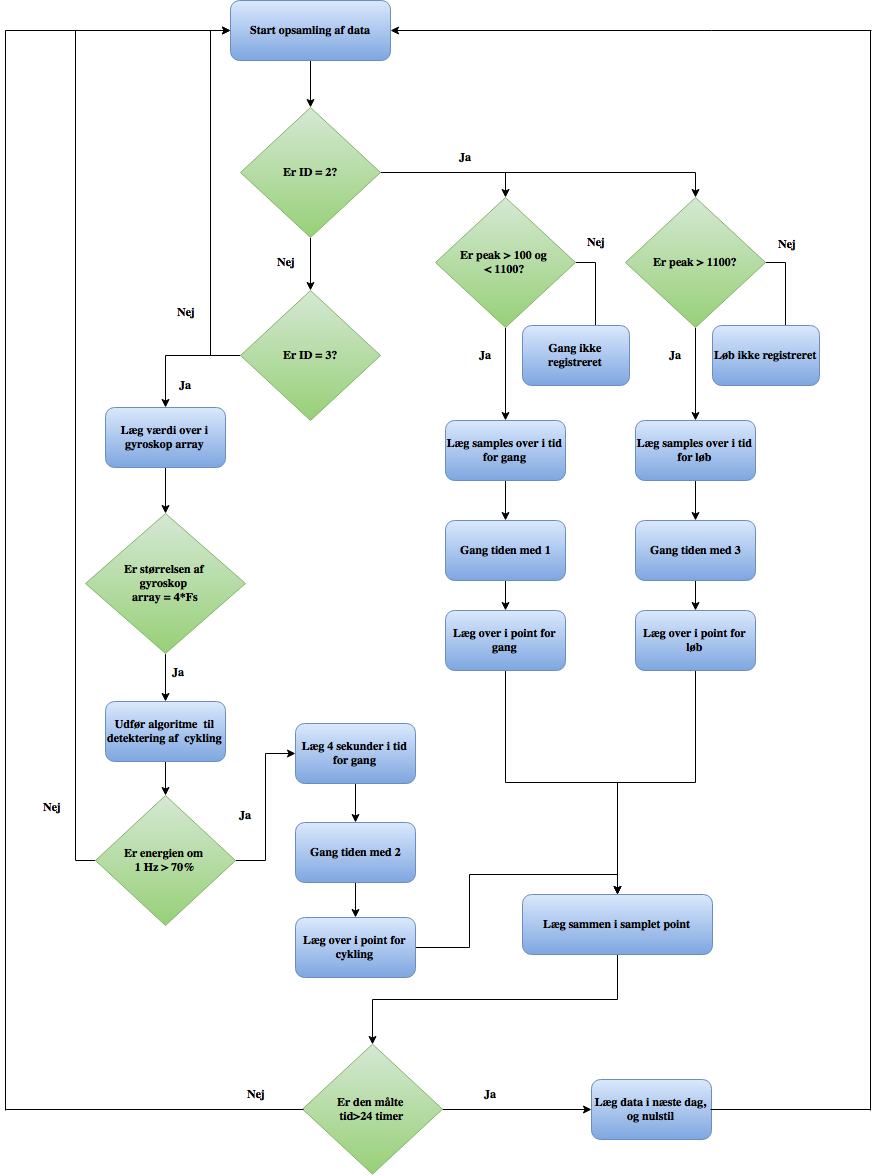
\includegraphics[scale=0.4]{figures/cDesign/pseudo_GUI.png}
	\caption{På figuren ses et flowchart som gennemgår hvorledes resultaterne fra de forskellige algoritmer behandles af GUI.}
	\label{fig:GUI}
\end{figure}

\subsection{Implementering}
GUI implementeres ved at anvende MATLABS funktion Graphical User Interface Design Environment (GUIDE). GUIDE er en funktion der gør det muligt at lave en specifik brugerflade med indbyggede funktioner.

Der indsættes en toggle button med teksten START, og når der trykkes på knappen, startes programmet, og teksten bliver ændret til STOP. Når programmet startes indhentes data fra mikrokontrolleren. \\
Er den første værdi to, registreres mikrokontrollerens array værende data fra accelerometeret. Den tredje værdi viderføres til løkker hvor det tjekkes hvorvidt det er et peak som repræsenteres af gang eller løb. Den anden værdi, som er en repræsentation af hvor mange samples der er mellem hvert peak, omregnes til minutter og lægges over i tidsvariablen for den pågældende aktivitet. Omregning udføres som \eqref{eq:tidsvariabel}. \\
Er den første værdi tre, registreres mikrokontrollerens array værende data fra gyroskopet. Den anden værdi fra mikrokontrolleren lægges derefter over i et array på 4*Fs, og behandles, som beskrevet i \secref{sec:algocykel}. En tidsvariabel på fire sekunder lægges derfor over i cykling, hvis databehandlingen viser at energien omkring 1~Hz er over 70 \%. 

\begin{equation}
\label{eq:tidsvariabel}
	tidsvariabel = tid/samplingsfrekvens*0,016667
\end{equation}

Derudover skal tidsvariablen omregnes til point, ved at multiplicere med de tidligere nævnte værdier opnået som følge af aktivitetstypen, som det ses på \eqref{eq:pointvariabel}. 
\begin{equation}
\label{eq:pointvariabel}
pointvariabel = tidsvariabel*aktivitetspoint
\end{equation}

Tidsvariablen og pointvariablen for de enkelte aktiviteter lægges over i forskellige static text felter, som tilhører henholdsvis point og tid for de tre forskellige aktivitetstyper. Ydermere er der to forskellige static text, hvor der i den ene samles tidsvariablerne for hele dagen, og i den anden samles point opnået gennem hele dagen. 
Derudover er der implementeret axis, hvor det er muligt at plotte data. I denne samles point fra cykling, gang og løb, som plottes oven på hinanden, hvormed det er muligt at se hvilke aktiviteter der er udført og hvor mange point de samlet set giver for en dag. 
I programmet er der aktiveret en timer, hvormed det er muligt at skifte mellem de forskellige dage efter 24 timer. Ved begyndelse på en ny dag nulstilles alle variabler, og der plottes i den næste dag. Slutteligt er der en reset toggle button, som gør det muligt at nulstille alt data. Denne er kun mulig at trykke på når programmet ikke kører. 

\subsection{Test}
Testen udføres med henhold til de opstillede krav og tilhørende tilladte afvigelser opstillet i \secref{krav_GUI}. Kravene beskriver, at GUI skal:
\begin{enumerate}
	\item Kunne visualisere tidsforbruget og point opnået ved henholdsvis gang, løb og cykling. 
\end{enumerate}


Testen udføres ved at indsende kendte værdier, hvoraf hver aktivitet kan testes individuelt i forhold til multiplikation som følge af aktivitetstype og intensitet.
Igennem testen indsendes et datasæt med simuleret input fra algoritmen, som skal trigge de forskellige aktiviteter. For gang indsendes [2 512 1100], for løb indsendes [2 512 1110] og for cykling indsendes [3 (35*sin(2$\pi$)*0,5*(2t))+60) 0]. De forskellige aktiviteter simuleres 60*6 gange, hvormed et simuleret signal på 6 minutter opnås.

Resultatet af GUIs design gør at forskellige aktivitetsformer bidrager til en forskellig mængde point. Ligeledes er varigheden og intensiteten  af aktiviteten afgørende for mængden af opnåede point, på baggrund af deres multiplikationsfaktor, hvilket kan ses i \eqref{eq:pointvariabel}
\begin{table}[H]
	\centering
	\begin{tabular}{ccc}
		\hline
		\rowcolor[HTML]{C0C0C0} 
		Aktivitet 	& Forventet antal point & Optalt antal point \\ \hline
		Gang 	  6 & 6	 \\ \hline
		Løb 	 18 & 18 \\ \hline
		Cykling  12 & 12 \\ \hline
	\end{tabular}
	\caption{I tabellen ses sammenhængen mellem forventede antal point og optalt antal point, som resultat af den indsendte simulerede data.}
	\label{test:GUI}
\end{table}\vspace{-.5cm}
På baggrund af testen af GUI, konkluderes det at denne fungerer efter hensigten. De forventede antal point og optalt antal point var nøjagtig det samme. Disse optjente point visualiseres i et søjlediagram som beskrevet i design. Varigheden af hvert aktivitet visualiseres som en værdi, der summeres op hver gang et aktivitetsresultat bliver behandlet. Resultatet af at indsende det simulerede data afspejlet i GUI kan ses på \figref{fig:GUI}.

\begin{figure}[H]
	\centering
	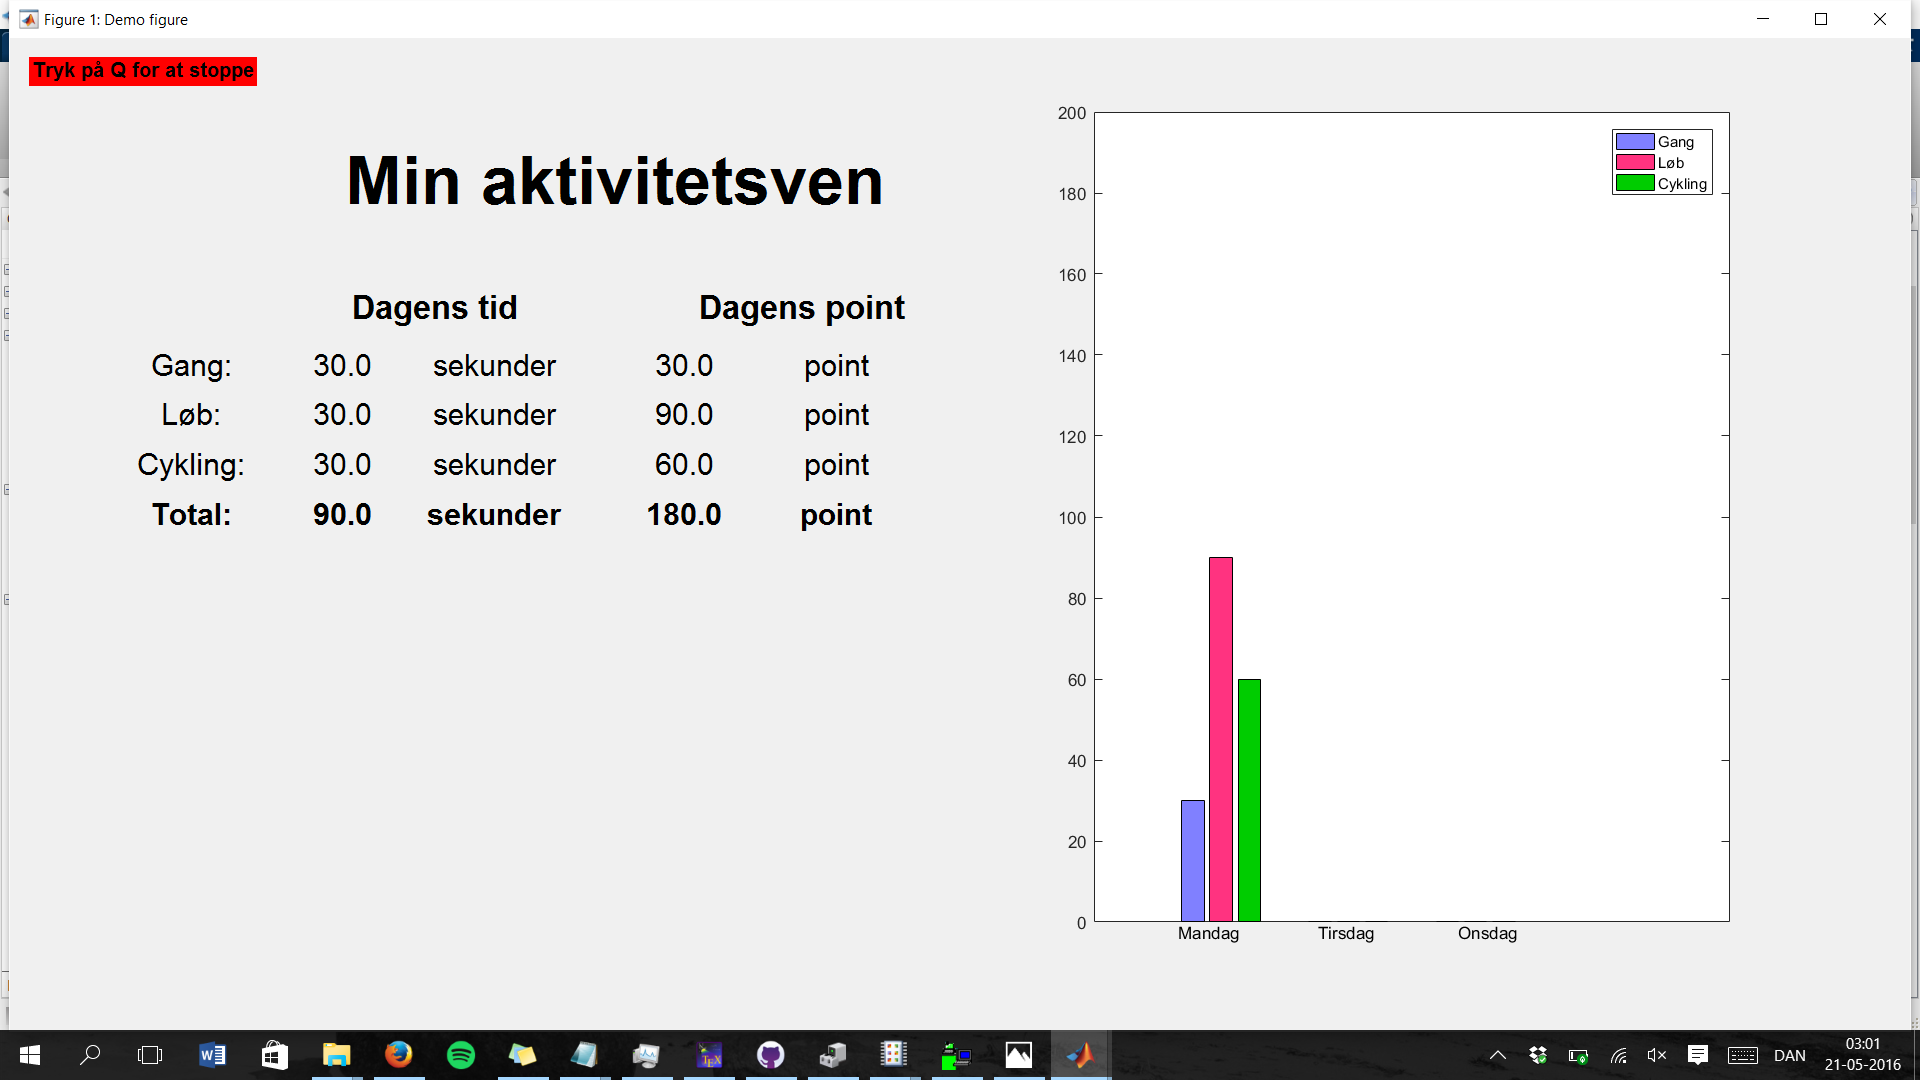
\includegraphics[scale=0.7]{figures/cDesign/test_GUI.png}
	\caption{På figuren ses et udklip af GUI hvor udførslen af aktiviteterne gang, løb og cykling visualiseres. Aktiviteternes samlede antal point og udført varighed ses på figuren.}
	\label{fig:GUI}
\end{figure}

Efterfulgt af design, implementering og test af GUI, kan det konkluderes at denne opfylder kravene heraf. GUI er i stand til at visualisere tidsforbruget samt antal point opnået, for alle aktiviteterne. GUI opdaterede kontinuert i testen hver gang et nyt input blev indsendt, hvoraf kravet vedrørende opdatering af GUI mindst hvert femtende minut, ligeledes er opfyldt.